\scanpage{69}
\mspage{30}
\uline{universal property} obvious for the morphisms
from \unsure{\unsure{this|the}|\deleted{\unsure{this|the}}} topological category $\uline{\Sigma}$ into a \inserted{pre}ordered set.
\S\ Suppose now that $\uline{\Sigma}$ satisfies the
% The two drafts below are cancelled by the actual stepped outline and
% three oblique strokes. Their running letters remain typeset text.
% No additional horizontal strike rules are supplied inside this drawing.
\figure{
\begin{tikzpicture}[x=1cm,y=-1cm, every node/.style={anchor=base west,inner sep=0pt,font=\small}]
\node at (0.23,0.66) {conditions};
\node at (2.28,1.03) {\inserted{c}};
\node at (4.24,0.45) {\unsure{a)} every invertible arrow of $\uline{\Sigma}$ is};
\node at (0.26,1.69) {an identity};
\node at (4.88,1.41) {a) \unsure{T|t}he map $\delta:\Sigma_0\unsure{\longrightarrow|-}\Sigma_1$ is};
\node at (0.19,2.64) {an open and closed embedding This is the case};
\node at (0.22,3.64) {if for example $\uline{b}:\Sigma_1\longrightarrow\Sigma_0$ is a proper};
\node at (0.10,4.73) {immersion....)};
\node at (3.65,4.29) {a) $\Sigma_{(1)}\overset{\uline{b}}{\unsure{-|\longrightarrow}}\Sigma_{(0)}$ is a proper};
\draw[line width=0.45pt]
 (13.98,0.29) .. controls (10.0,0.17) and (6.9,0.34) .. (4.24,0.46)
 -- (4.07,1.52) -- (0.32,1.58)
 -- (0.05,4.84) -- (3.06,4.60) -- (2.92,3.75)
 -- (13.43,3.08);
\draw[line width=0.45pt] (1.85,4.08) .. controls (1.60,4.28) and (1.61,4.08) .. (1.70,3.95) -- (2.68,2.10);
\draw[line width=0.45pt] (5.49,2.83) .. controls (5.22,3.02) and (5.23,2.97) .. (5.32,2.87) -- (6.64,0.62);
\draw[line width=0.45pt] (8.65,2.14) -- (9.53,0.51);
\end{tikzpicture}
}
immersion ($\Longrightarrow\ \delta:\Sigma_{(0)}\unsure{-|\longrightarrow}\Sigma_{(1)}$ is an open
and closed immersion, so that \deleted{$\Sigma_{(1)}=\delta(\Sigma_{(0)})\amalg$}
\[
\Sigma(1)\simeq\delta(\Sigma(0))\amalg\Sigma^{*}(1)
\quad )
\]

b) $\Sigma^{*}(1)\xrightarrow{\uline{b}|\Sigma^{\unsure{\prime|*}}(1)}\Sigma(0)$ is an immersion with
locally \uline{nowhere dense} image ie : empty interior...

c) \deleted{\unsure{---}} Every connected component of $\Sigma_{(0)}$ is of
finite dimension.
Then one finds that $\Sigma_{ii}^{*}\overset{\mathrm{definition}}{=}\Sigma_{ii}\cap\Sigma^{\unsure{\prime|*}}(1)=\varnothing$,
for reasons of dimension (for $\Sigma_{ii}^{\unsure{*|<}}$ is
fibered over \unsure{over|\deleted{over}} $\Sigma_i$, hence if it is nonempty, of
dimension $\geq\dim\Sigma_i$; but since $\Sigma_{ii}^{\unsure{*|<}}\unsure{-|\longrightarrow}\Sigma_i^{\unsure{\wedge|*}}$ is
a nowhere dense immersion, one must also have $\dim\Sigma_{ii}^{\unsure{*|<}}<$
$\dim\Sigma_i^{*}$, so $\Sigma_{ii}^{<}$ is empty), i.e.
\par\noindent
\begin{tikzpicture}[baseline=(f.base),x=0.01cm,y=-0.01cm]
\node[inner sep=0pt] (f) at (169,81) {$\Sigma_i\xrightarrow{\sim}\Sigma_{ii}$};
\draw[line width=0.45pt] (9,17) .. controls (120,17) and (220,8) .. (330,5);
\draw[line width=0.45pt] (7,32) -- (8,127) -- (330,118) -- (333,29);
\end{tikzpicture}: every arrow \deleted{in} between two
\deleted{\unsure{objects} of} elements of $\Sigma_{(0)}$ that are in the
same connected component \deleted{\unsure{are|is}} is an identity.
\margin{\handwritten{68}}
